\documentclass{ltjsarticle}
\usepackage{amsmath}
\usepackage{amssymb}
\usepackage{ascmac}
\usepackage[dvipdfmx]{graphicx}
\usepackage[colorlinks=true, allcolors=blue]{hyperref}
\usepackage{fancybox}

\begin{document}

\title{機械学習}
\author{秋葉洋哉}
\maketitle
\section{導入}
\subsection{機械学習とは}
トム・ミッチェル (1997) によれば、コンピュータプログラムにおいて、タスクTを性能指標Pで測定し、経験Eから学習させ、このとき性能指標Pが最大となるように学習を繰り返すことが機械学習である。

\subsection{機械学習のモデリングプロセス}
機械学習のモデリングプロセスは以下のようになる。
\begin{enumerate}
  \item 問題設定
  \item データ選定
  \item データ前処理
  \item 機械学習・モデル選択
  \item モデル学習
  \item モデル評価・改良
\end{enumerate}
ビジネスにおいて、最も大切なプロセスが問題設定の部分であり、機械学習を用いるかどうか、という点をまず第一に考える必要がある。

\subsection{機械学習の分類}
機械学習は、学習種類・タスク・アルゴリズム(パラメータの推定問題)の3つの観点から分類される。
\begin{enumerate}
  \item 学習種類
  \begin{itemize}
    \item 教師あり学習
    \item 教師なし学習
  \end{itemize}
  \item タスク
  \begin{itemize}
    \item 予測 (回帰)
    \item 分類
    \item クラスタリング
    \item 次元削減
  \end{itemize}
  \item アルゴリズム
  \begin{itemize}
    \item 線形・非線形回帰 (最小二乗法・尤度最大化)
    \item ロジスティック回帰 (尤度最大化)
    \item サポートベクターマシン (マージン最大化)
    \item K-means
    \item 主成分分析 (分散最大化)
  \end{itemize}
\end{enumerate}

\newpage

\section{線形回帰モデル}
\subsection{概要}
線形とは、比例の関係である状態のことであり、線形回帰モデルは、入力変数と出力変数の関係が線形であると仮定した時の回帰モデルである。
n次元の線形回帰モデルは、$a_k$, $x_k$を用いて以下のように表される。
\begin{align}
  y &= a_0 + a_1x_1 + a_2x_2 + \cdots + a_{n-1}x_{n-1}\\
  &= a_0 + \sum_{k=1}^{n-1}a_{k} x_{k}\\
  &= \sum_{k=1}^{n-1}a_{k} x_{k} \quad\text{,where $x_0 = 1$}\\
  &= \boldsymbol{a}^T\boldsymbol{x}
\end{align}
ただし、$\boldsymbol{a} = (a_0, a_1, \cdots, a_{n-1})^T$, $\boldsymbol{x} = (1, x_1, x_2, \cdots, x_{n-1})^T$である。
\par
回帰問題とは、ある入力から連続値の出力を予測する問題のことで、直線で予測されるなら線形回帰モデル、曲線で予測されるなら非線形回帰モデルが用いられる。
\par
本来解きたい問題よりも、難しい問題にして解決しようとせずに、解きたい問題よりも簡単な問題にして解決するほうがよい、というエンジニアリング上の教訓がある。これは、Vapnicの原理と呼ばれている。
回帰分析を用いることで、例えば何かの順位を予測することは可能である。ただし、解きたい問題が順位を決める、という問題である場合、回析分析を用いることは適切ではない。なぜなら、回帰分析では、順位だけではなく、順位の間隔も予測することになるため、解きたい問題よりも難しい問題になってしまうからである。
つまり、回帰分析を用いる場合は、解きたい問題が何かを明確にし、連続値として予測される問題であれば使用することが適切である。
\par
回帰 (さしずめ機械学習) においては、入力値を説明変数、出力値を目的変数と呼ぶ。説明変数は特徴量とも呼ばれる。
回帰分析では、説明変数と目的変数の関係を表すモデルを構築し、そのモデルを用いて目的変数を予測する。
回帰分析は、教師あり学習の一つで、入力とm次元パラメータの線形結合を出力するモデルである。
式で表すと、
\begin{align}
  y &= \boldsymbol{w}^T\boldsymbol{x} + w_0 + \epsilon_i\\
  &= \sum_{k=1}^{m}w_{k} x_{k} + w_0 + \epsilon_i
\end{align}
ただし、$\epsilon_i$は誤差項である。
で表すことができる。
これを図で表すと、図\ref{fig:kaiki}のようになる。
\begin{figure}[htbp]
  \centering
  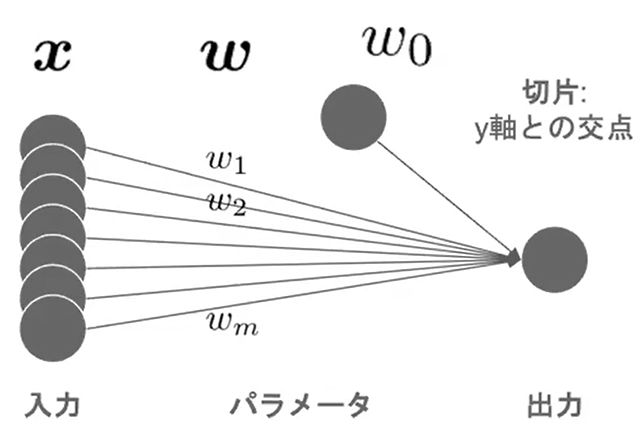
\includegraphics[width=10cm]{kaiki.png}
  \caption{線形回帰モデルの概念図}
  \label{fig:kaiki}
\end{figure}

数式のそれぞれを説明した図が、図\ref{fig:equation}である。
\begin{figure}[htbp]
  \centering
  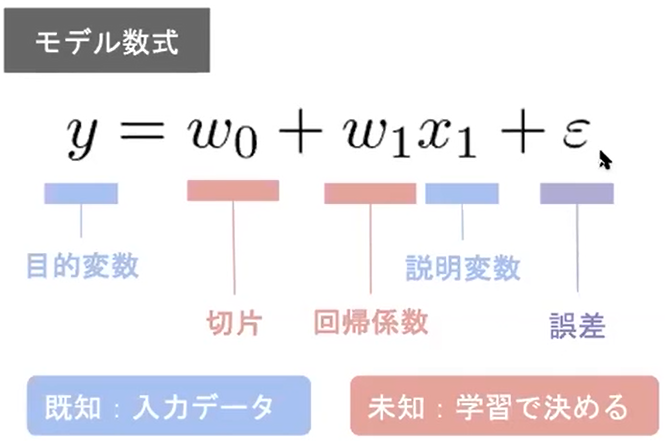
\includegraphics[width=10cm]{equation.png}
  \caption{線形回帰モデル式のそれぞれの意味}
  \label{fig:equation}
\end{figure}
図\ref{fig:equation}における誤差は、$x_1$以外の要素があるとき、本来は$x_2$, $x_3$を用いて多次元にすべき部分が定数として収められた部分になる。

また、誤差項$\epsilon_i$は、平均0、分散$\sigma^2$の正規分布に従うと仮定して、モデルの不完全的要素を表す。この仮定に基づいて、最尤推定法を用いてパラメータを推定する。

\subsection{汎化}
機械学習において、学習データに対して過度に適合してしまうことを過学習と呼び、未知のデータに対しても適切に予測できることを汎化と呼ぶ。
過学習を防ぐためには、学習データを訓練データとテストデータに分割し、訓練データで学習を行い、テストデータで評価を行うことが一般的である。

\newpage

\subsection{最小二乗法}
最小二乗法は、誤差の二乗和を最小にするようなパラメータを求める方法である。
学習データを用いて、誤差の二乗和を最小にするようなパラメータを求めることで、モデルのパラメータを最適化することができる。
式で表すと、
\begin{align}
  \text{MSE}_{\text{train}}(\boldsymbol{w}) &= \frac{1}{n_\text{train}}\sum_{i=1}^{n_\text{train}}(\hat{y_i} - y_i)^2\\
  &= \frac{1}{n_\text{train}}\sum_{i=1}^{n_\text{train}}(\boldsymbol{x}^T_i \boldsymbol{w} - y_i)^2
\end{align}
で表すことができる。ただし、$\hat{y_i}$は予測値、$y_i$は実測値、$n_\text{train}$は学習データの数である。
この式を最小にするようなm次元の$\boldsymbol{w}$の組み合わせを求めることが、線形回帰モデルを作成する上での目標である。
最小二乗法は、一般的に外れ値の影響を受けやすいという欠点があるたけ、外れ値を多く含むデータに対しては、前処理を工夫したり、Huber損失、Tukey損失(外れ値無視)などのロバスト回帰を用いることがある。
\par
MSEを最小にするようなm次元の$w$を求める、という部分は数式では
\begin{align}
  \hat{w} = \arg\min_{w\in \mathbb{R}^{m+1}}\text{MSE}_{\text{train}}(w)
\end{align}
と表すことができる。この$\hat{w}$を求めることが最小二乗法の目標である。
そのためには、MSEを$w$で微分し、その微分が0になるような$w$を求めることが必要である。つまり、
\begin{align}
  \frac{\partial}{\partial w}\text{MSE}_{\text{train}}(w) = 0
\end{align}
を解くことで、最小二乗法によるパラメータの最適化を行うことができる。
\iffalse
実際にこの微分式を解いてみる。
\begin{align}
  & \frac{\partial}{\partial w}\text{MSE}_{\text{train}}(w) = 0\\
  &\Rightarrow \frac{\partial}{\partial w} { \frac{1}{n_{\text{train}}} \sum_{i=1}^{n_{\text{train}}} (\hat{y}_i - y_i)^2 } = 0\\
  &\Rightarrow \frac{\partial}{\partial w}{ \frac{1}{n_\text{train}}\sum_{i=1}^{n_\text{train}}(\boldsymbol{x}^T_i \boldsymbol{w} - y_i)^2} = 0\\
  &\Rightarrow \frac{\partial}{\partial w}{ \frac{1}{n_\text{train}} (\boldsymbol{X}\boldsymbol{w} - \boldsymbol{y})^T (\boldsymbol{X}\boldsymbol{w} - \boldsymbol{y})} = 0
\end{align}
ここで、$(\boldsymbol{X}\boldsymbol{w} - \boldsymbol{y})$を具体的に行列を用いて表すと、
\begin{align}
  \begin{pmatrix}
    \boldsymbol{x}^T_1\\
    \boldsymbol{x}^T_2\\
    \vdots\\
    \boldsymbol{x}^T_{n_{\text{train}}}
  \end{pmatrix}
 \cdot
  \begin{pmatrix}
    w_1\\
    w_2\\
    \vdots\\
    w_{n_{\text{train}}}
  \end{pmatrix}
=
  \begin{pmatrix}
    y_1\\
    y_2\\
    \vdots\\
    y_{n_{\text{train}}}
  \end{pmatrix}
\end{align}
\fi

\begin{figure}[htbp]
  \centering
  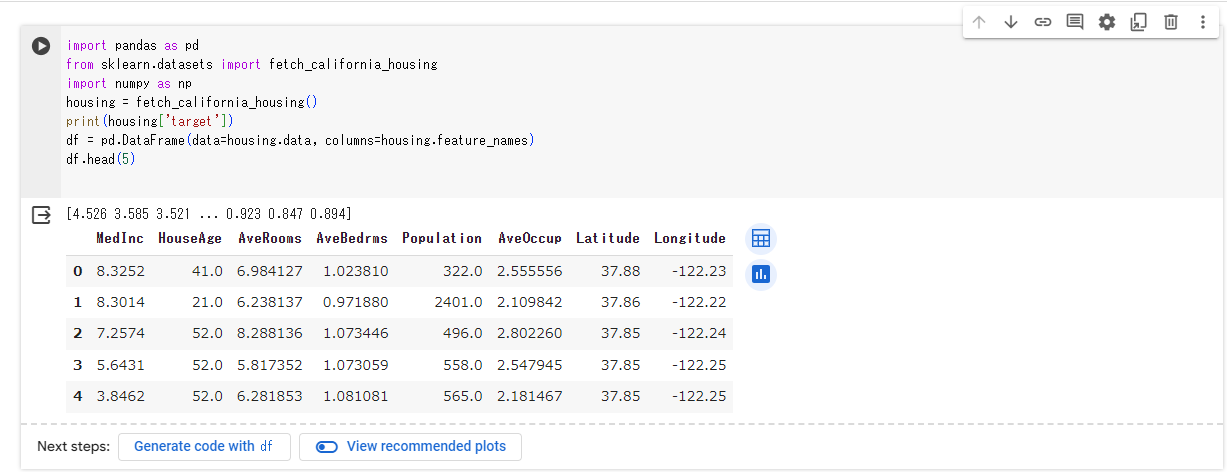
\includegraphics[width=12cm]{capture/cap_1.png}
  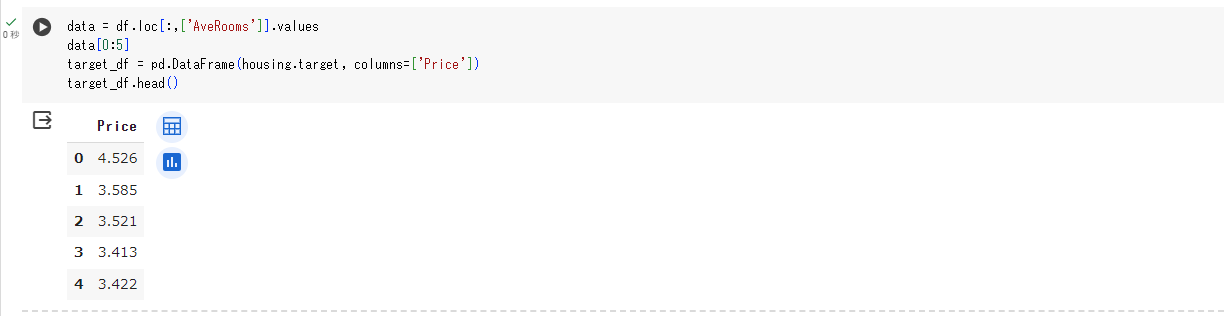
\includegraphics[width=12cm]{capture/cap_2.png}
  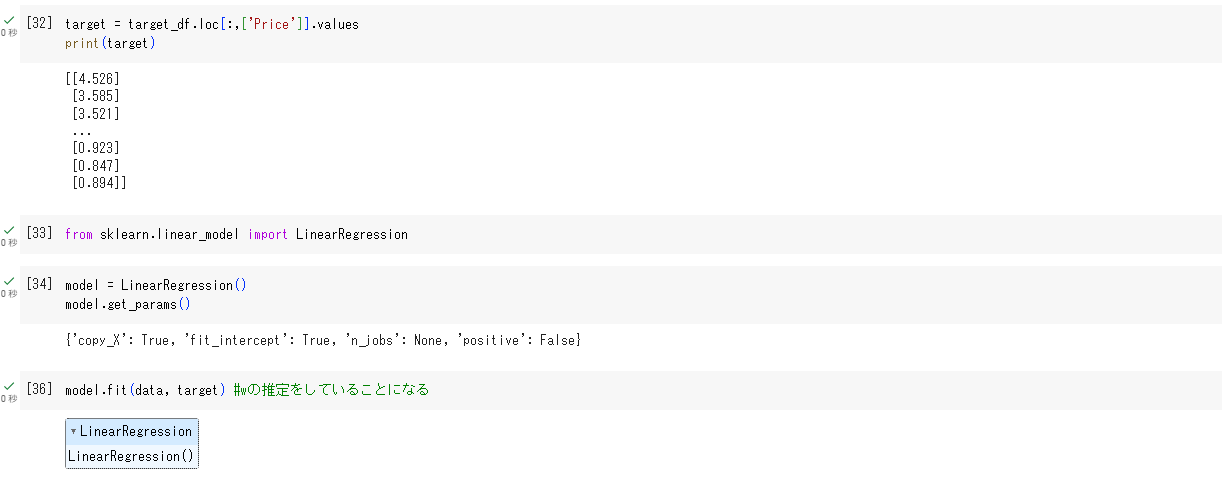
\includegraphics[width=12cm]{capture/cap_3.png}
  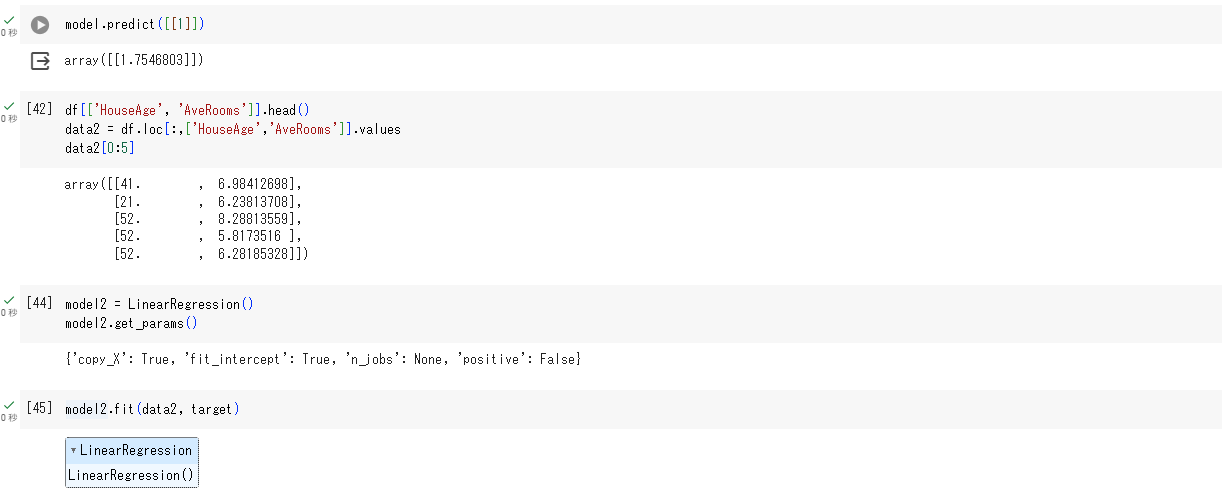
\includegraphics[width=12cm]{capture/cap_4.png}
  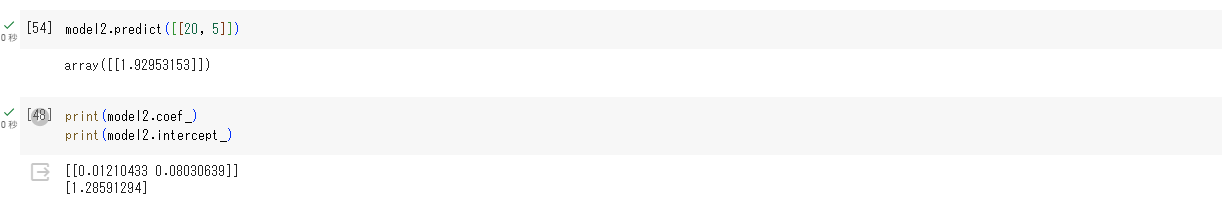
\includegraphics[width=12cm]{capture/cap_5.png}
  \caption{実装演習キャプチャ (カリフォルニアデータセットで代用)}
\end{figure}

\newpage

\section{非線形回帰モデル}
\subsection{概要}
非線形回帰とは、例えば、以下のような関数を用いて回帰を行う。
\begin{align}
  y &= w_0 + w_1x + w_2x^2 + w_3x-3\\
  y &= w_0 + w_1\sin(x) + w_2\cos(x) + w_3\log(x)
\end{align}
非線形回帰モデルは、線形回帰における$x$という変数部分を$\phi(x)$で置き換えたものと考えることができる。
従って、線形回帰における重み$\mathbf{w}$の導出を、非線形回帰においても適用することができる。
\begin{align}
  \hat{y} = w_0 + w_1\phi(x_1) + w_2\phi(x_2) + \cdots + w_m\phi(x_m)
\end{align}
このようにして展開する方法を、基底展開法と呼ぶ。
このことは、重み$\mathbf{w}$について線形であるということができる。
ただし、$\phi(x)$は基底関数と呼ばれる関数で、多項式関数、ガウス基底関数、シグモイド基底関数などがある。
多項式関数は、
\begin{align}
  \phi(x) = x^j
\end{align}
で表される。ガウス基底関数は、
\begin{align}
  \phi(x) = \exp\left(-\frac{(x-\mu_j)^2}{2\sigma^2}\right)
\end{align}
で表される。
ガウス基底関数は、2つの山を考え、それぞれの山の中心を$\mu_1$, $\mu_2$とし、それぞれの山の広がりを$\sigma_1$, $\sigma_2$とすることで、ある入力が与えられたとき、それがどちらの山の影響を強く受けるかを表すことができる。
\begin{figure}[htbp]
  \centering
  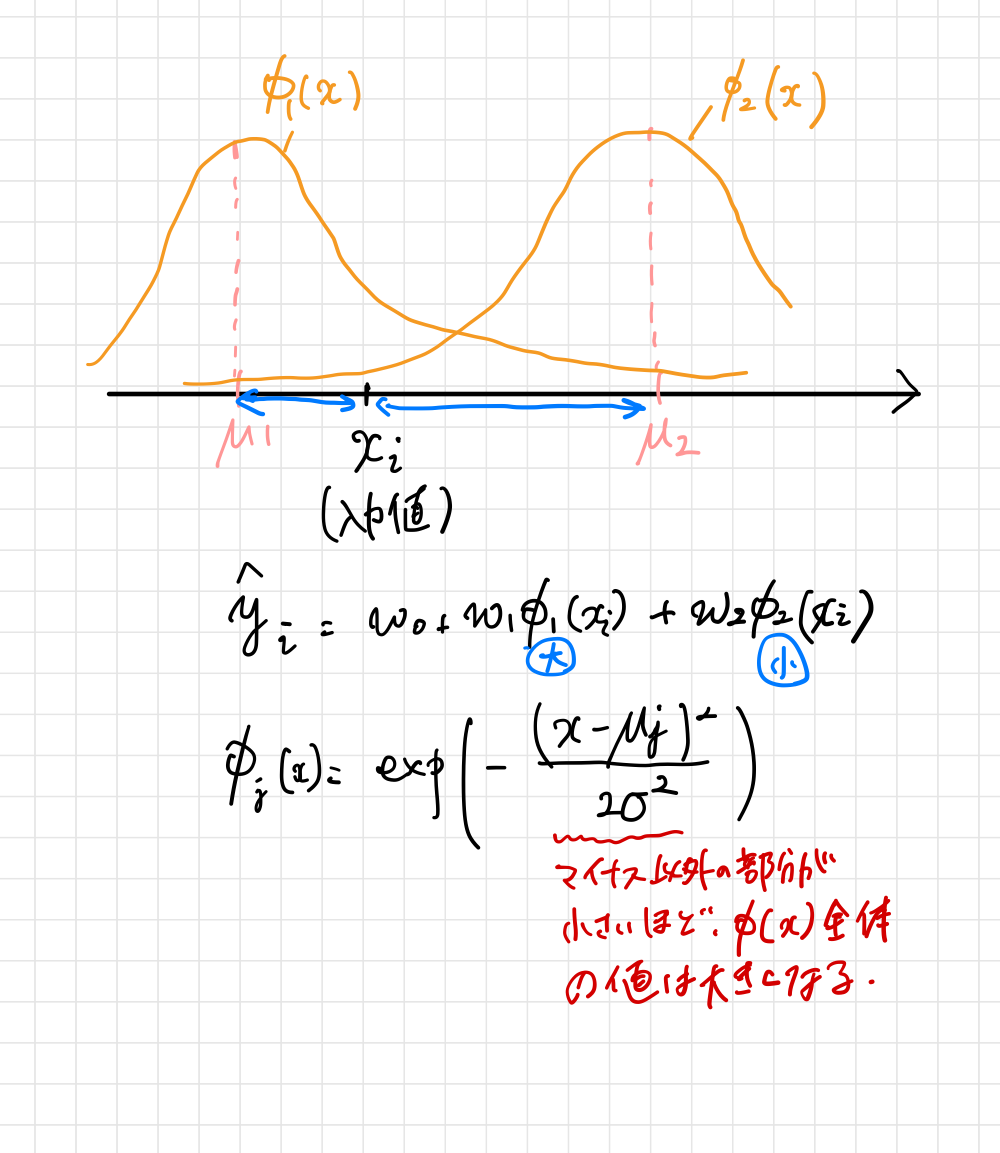
\includegraphics[width=12cm]{capture/ガウス基底関数.png}
  \caption{ガウス基底関数のイメージ}
\end{figure}
シグモイド基底関数は、
\begin{align}
  \phi(x) = \frac{1}{1+\exp(-\beta(x-\mu))}
\end{align}
で表される。

線形回帰における行列表記を、非線形回帰に適応させると、
\begin{align}
  \boldsymbol{y} = \boldsymbol{X}\boldsymbol{w}
\end{align}
が、
\begin{align}
  \boldsymbol{y} = \boldsymbol{\Phi}\boldsymbol{w}
\end{align}
となる。ただし、$\boldsymbol{\Phi}$は、
\begin{align}
  \boldsymbol{\Phi} = 
  \begin{pmatrix}
    \phi(x_1) & \phi(x_2) & \cdots & \phi(x_m)
  \end{pmatrix}
\end{align}
である。
結局、MSEを最小化する$\boldsymbol{w}$は、$\boldsymbol{X}$を$\boldsymbol{\Phi}$に置き換えるだけで、
\begin{align}
  \hat{\boldsymbol{w}} = \Phi^T(\Phi\Phi^T)^{-1}\boldsymbol{y}
\end{align}
となる。

\newpage

\subsection{未学習と過学習}
未学習とは、学習データに対しても適合が悪い状態のことであり、過学習とは、学習データに対して過度に適合してしまう状態のことである。
過学習を防止する策として、以下が挙げられる。
\begin{enumerate}
  \item 学習データを増やす
  \item 使用する説明変数を減らす
  \item 正則化を行う
\end{enumerate}
正則化については、以下のように考える。
線形回帰における、予測$\hat{y}$は、
\begin{align}
  \hat{y} = X_{\star} \cdot (\boldsymbol{X}^T\boldsymbol{X})^{-1}\boldsymbol{X}^T\boldsymbol{y}
\end{align}
であった。ただし、$(\boldsymbol{X}^T\boldsymbol{X})^{-1}\boldsymbol{X}^T\boldsymbol{y}$は、$\boldsymbol{w}$である。過学習を防ぐということは、あまりにも$\boldsymbol{w}$が大きくなりすぎないようにすることである。
つまり、$(\boldsymbol{X}^T\boldsymbol{X})^{-1}$が大きくなりすぎないようにすることが必要である。
例えば、ある入力値$\boldsymbol{X}$が
\begin{align}
 \boldsymbol{X} = 
  \begin{pmatrix}
    1 & 2 & 4 \\
    1 & 3 & 5.9\\
    1 & 4 & 8.1\\
  \end{pmatrix}
\end{align}
であるとする。この3番目のベクトルが、2番目のベクトルとほぼ同じであると考えられる。これは、2本のベクトルが平行に近いことを意味している。
このような場合、転置行列を前から掛けた時の行列は、
\begin{align}
  \boldsymbol{X}^T\boldsymbol{X} = 
  \begin{pmatrix}
    1 & 1 & 1\\
    2 & 3 & 4\\
    4 & 5.9 & 8.1\\
  \end{pmatrix}
  \begin{pmatrix}
    1 & 2 & 4 \\
    1 & 3 & 5.9\\
    1 & 4 & 8.1\\
  \end{pmatrix}
  =
  \begin{pmatrix}
    3 & 9 & 18\\
    9 & 29 & 58.1\\
    18 & 58.1 & 116.42\\ 
  \end{pmatrix}
\end{align}
であるから、
逆行列は、
\begin{align}
  (\boldsymbol{X}^T\boldsymbol{X})^{-1} = 
  \begin{pmatrix}
    3 & 9 & 18\\
    9 & 29 & 58.1\\
    18 & 58.1 & 116.42\\ 
  \end{pmatrix}^{-1}
  \approx
  \begin{pmatrix}
    6.33 & -22 & 10\\
    -22 & 281 & -137\\
    10 & -137 & 66.7\\
  \end{pmatrix}
\end{align}
となる。本来であれば、大きくても2桁程度の値に収まるべきであるが、この逆行列は、数値が大きくなりすぎている。
よって、$\boldsymbol{w}$が大きな値を取ることとなり、過学習を引き起こすこととなる。
これを防ぐために、MSE最小化に対して、罰則化項を導入することで、$\boldsymbol{w}$が大きな値を取らないようにすることができる。
\begin{align}
  E(\boldsymbol{w}) = \text{MSE}_{\text{train}}(\boldsymbol{w}) + \lambda \boldsymbol{w}^T\boldsymbol{w}
\end{align}
ただし、E($\boldsymbol{w}$)は、正則化項を導入した誤差関数で、$\lambda$は正則化項の重みである。この2項目で、$\boldsymbol{w}$が大きな値を取った時に、誤差が大きくなるようになり、MSEを最小化するという目的に対して、$\boldsymbol{w}$が大きな値を取らないようにするという仕組みである。

このような最適化の流れを一般化すると、以下で表される。
解きたいものは、$R(\boldsymbol{w}) \le r$ という条件を満たしつつ、$min \text{MSE}$を求めることである。
そこで、KKT条件を用いて、以下のように最適化問題を解くことができる。
\begin{align}
  min \text{MSE}  + \lambda R(\boldsymbol{w})\\
\end{align}
この第2項目部分によって不等式条件を満たすことができる。

回帰分析におけるRidge回帰と、Lasso回帰は、どちらも正則化項を導入することで、過学習を防ぐ方法であるが、Ridge回帰は、L2正則化を行い、Lasso回帰は、L1正則化を行うという説明がなされることが多い。
そのうち、L2正則化というものが$\lambda \boldsymbol{w}^T\boldsymbol{w}$を使用する方法になる。

\begin{figure}[htbp]
  \centering
  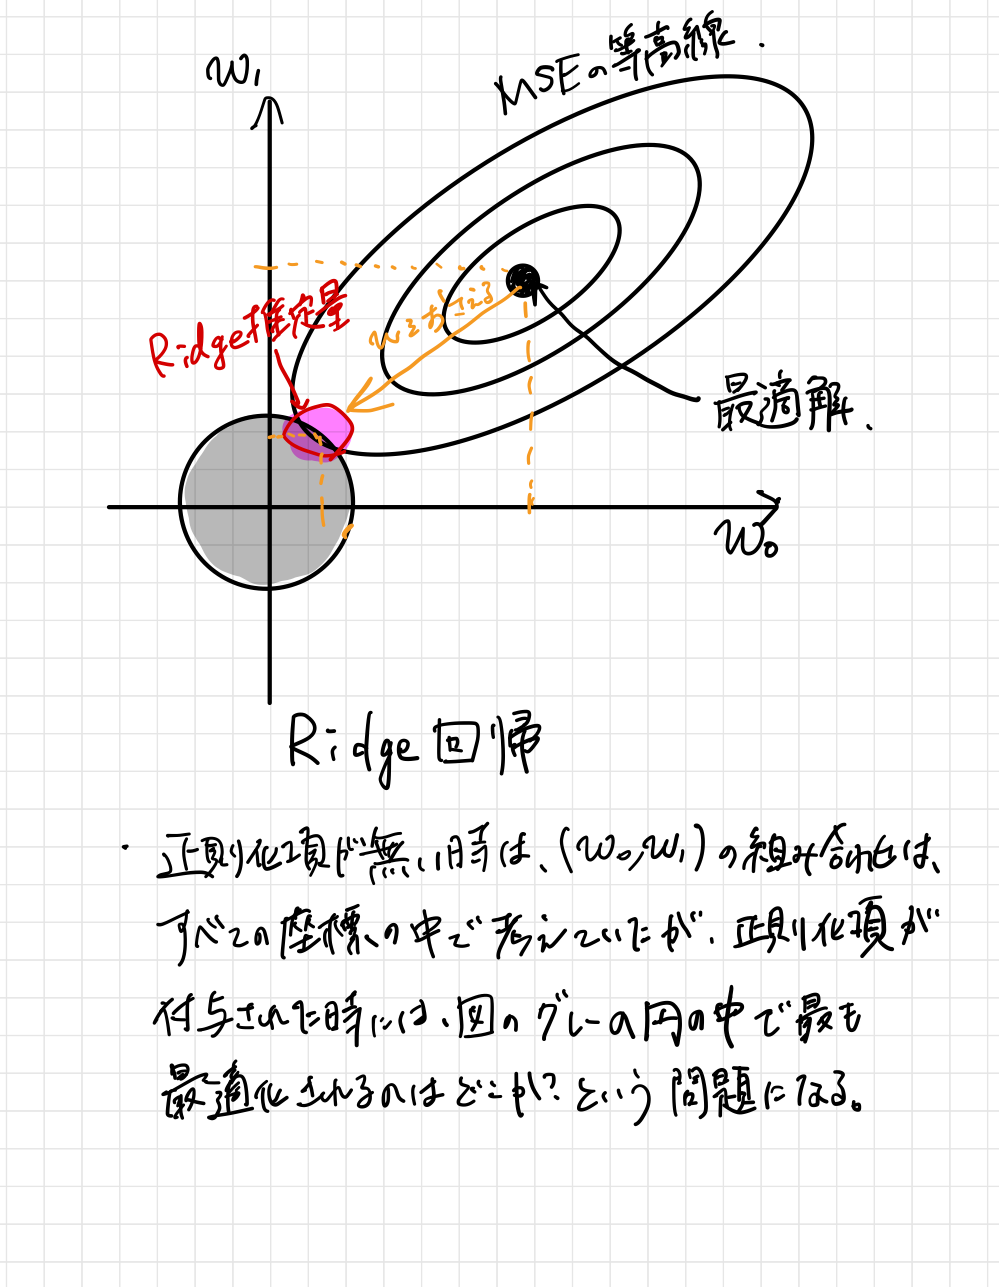
\includegraphics[width=13cm]{capture/Ridge回帰.png}
  \caption{Ridge回帰のイメージ}
\end{figure}

\newpage

\subsection{学習と検証}
学習と検証は、モデルの汎化性能を評価するための方法である。
\par
ホールドアウト法は、データを訓練データとテストデータに分割し、訓練データで学習を行い、テストデータで評価を行う方法である。一括でデータを分割するため、データの偏りが生じる可能性がある。例えば、検証データ内に外れ値が含まれてしまうと、モデルの評価が不正確になる可能性がある。
\par
クロスバリデーション (交差検証) は、データをk個に分割し、k-1個のデータで学習を行い、残りの1個のデータで評価を行う方法である。この操作をk回繰り返し、k個の評価結果の平均を取ることで、モデルの評価を行うことができる。
交差検証は、ホールドアウト法に比べて、データの偏りが生じにくいという利点がある。
\par
グリッドサーチは、ハイパーパラメータの最適な値を探索するための方法である。ハイパーパラメータとは、モデルの学習時に設定するパラメータのことで、例えば、正則化項の重み$\lambda$や、基底関数の次数などがある。

\newpage

\section{ロジスティクス回帰}
\subsection{概要}
以降では、分類における問題を考える。
分類においては、識別的アプローチと生成的アプローチの2つのアプローチがある。
\begin{itemize}
  \item 識別的アプローチ: ある入力に対して、その入力がどのクラスに属するかを直接予測する方法。例えば、ロジスティック回帰、SVM、決定木などがある。$P(C_k)$が求めたいクラスの確率とすると、$P(C_k|\boldsymbol{x})$を直接モデル化して求める。
  \item 生成的アプローチ: ある入力が与えられた時に、その入力が生成される確率を求め、その確率が最大となるクラスを予測する方法。例えば、ナイーブベイズ、GMM、HMMなどがある。つまり、$P(C_k)$, $P(\boldsymbol{x}|C_k)$をモデル化し、その後、ベイズの定理を用いて$P(C_k|\boldsymbol{x})$を求める。
\end{itemize}
識別的アプローチにおいては、分類される確率の最も高いクラス$\hat{y}$を求めることが目的であり、
\begin{align}
  \hat{y} = \arg \max_{k} P(C_k|\boldsymbol{x})
\end{align}
を解くことで求める。一方で、生成的アプローチにおいては、$P(\boldsymbol{x})$の確率は一定であるため、
\begin{align}
  \hat{y} = \arg \max_{k} P(C_k)P(\boldsymbol{x}|C_k)
\end{align}
を解くことで求める。ここで、$P(C_k)$は各クラスの割合である (例えば、クラス1の確率が60\%なら$P(C_k)=0.6$)。$P(\boldsymbol{x}|C_k)$は、「各クラスが観測データ$x$を生成する確率 (尤度) がどのくらいであるか」を表したものである。このようにすることで、あるクラスに属する疑似的なデータを生成することができるという利点がある。

ロジスティック回帰は、識別的アプローチに属する手法で、入力が与えられた時に、その入力がどのクラスに属するかを直接予測する方法である。

回帰分析では、実数全体から実数全体への関数を求めるため、
\begin{align}
  \boldsymbol{w}^T\boldsymbol{x} \in \mathbb{R}
\end{align}
であったが、ロジスティック回帰では、実数全体から0, 1の2値への関数を求めるため、
\begin{align}
  \sigma(\boldsymbol{w}^T\boldsymbol{x}) \in [0, 1]
\end{align}
を考える。ただし、$\sigma$はシグモイド関数で、
\begin{align}
  \sigma(z) = \frac{1}{1+\exp(-z)}
\end{align}
で表される。
このシグモイド関数は、$z$が大きいときに1に近づき、$z$が小さいときに0に近づく性質を持つ。
この性質を用いて、入力が与えられた時に、その入力がどのクラスに属するかを予測することができる。
\begin{figure}[htbp]
  \centering
  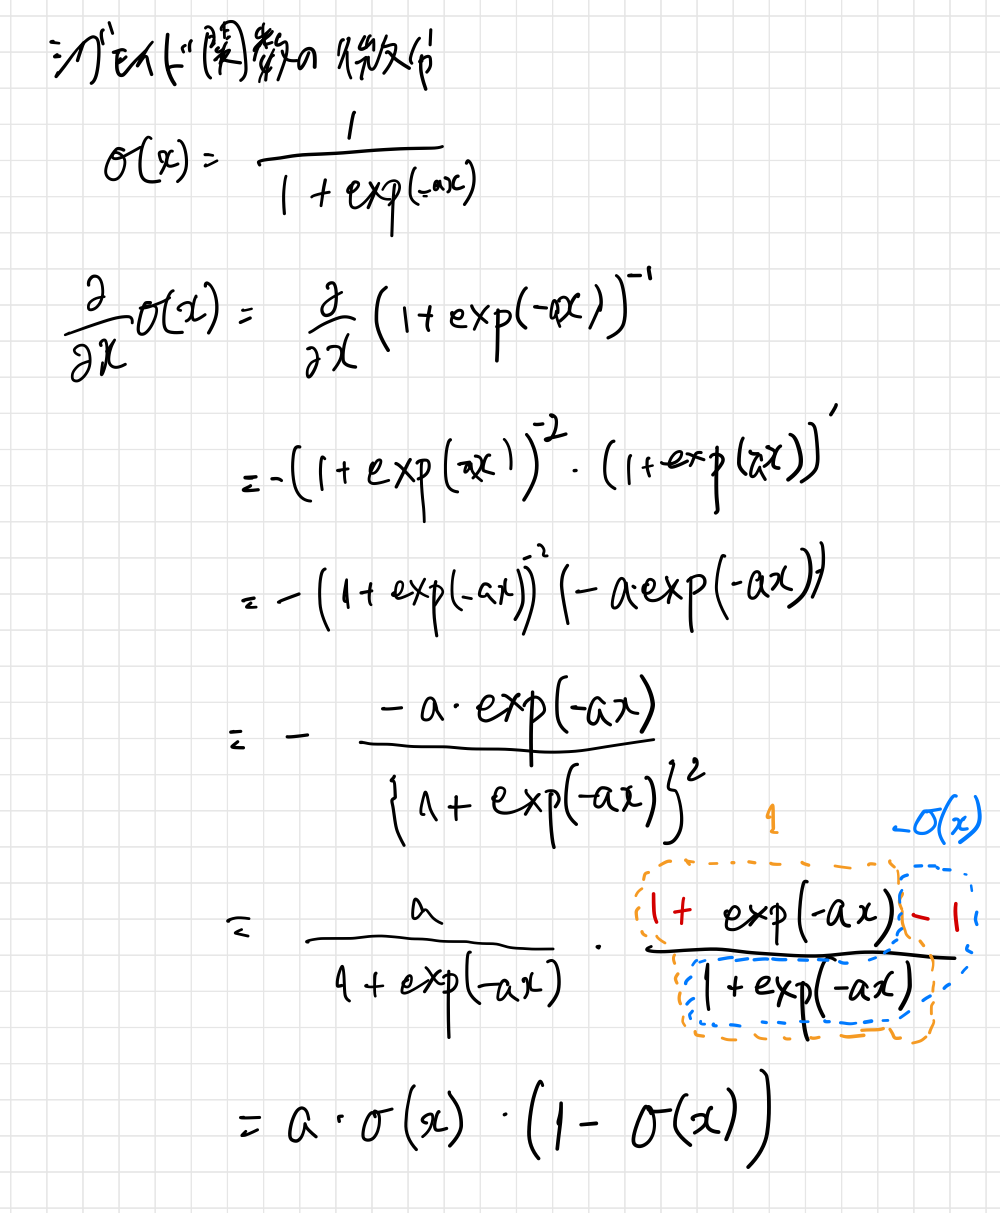
\includegraphics[width=13cm]{capture/シグモイド関数の微分.png}
  \caption{シグモイド関数の微分}
\end{figure}

\newpage

\subsection{最尤推定}
ある分布を仮定した時に、その分布が観測データを生成する確率が最大となるようなパラメータを求める方法を最尤推定と呼ぶ。データは固定されたものとして、パラメータを変化させることで、尤度を最大化するようなパラメータを求めるアプローチである。
ロジスティック回帰においては、尤度関数は、
\begin{align}
  L(\boldsymbol{w}) &= \prod_{i=1}^{n}P(C_k|\boldsymbol{x}_i)^{y_i}(1-P(C_k|\boldsymbol{x}_i))^{1-y_i} \\
&= \prod_{i=1}^{n}\sigma(\boldsymbol{w}^T\boldsymbol{x}_i)^{y_i}(1-\sigma(\boldsymbol{w}^T\boldsymbol{x}_i))^{1-y_i}  
\end{align}
で表される。ただし、$y_i$は、$i$番目のデータがクラス$C_k$に属するかどうかを表すラベルである。尤度関数では、確率変数が独立かつ同一の分布に従っていることを仮定しているため、各データの確率の積として表されている。
この尤度関数を最大化するようなパラメータ$\boldsymbol{w}$を求めることが、ロジスティック回帰における最尤推定の目標である。
ただし、尤度関数をそのまま最大化することは難しいため、尤度関数の対数を取り、対数尤度関数を最大化することが一般的である。
対数尤度関数は、
\begin{align}
  \log L(\boldsymbol{w}) &= \sum_{i=1}^{n}\{y_i\log \sigma(\boldsymbol{w}^T\boldsymbol{x}_i) + (1-y_i)\log(1-\sigma(\boldsymbol{w}^T\boldsymbol{x}_i))\}
\end{align}
で表される。
\begin{itembox}[l]{なぜ対数尤度関数を用いるのか?}
  尤度関数は確率の掛け算で表されている。1よりも小さい値の確率の掛け算を繰り返すことで、とても小さな値となって計算機でオーバーフローが発生する可能性があるため、対数を用いて積を和に、指数を積に変換することで、計算を安定化させることができる。
\end{itembox}

\begin{figure}[htbp]
  \centering
  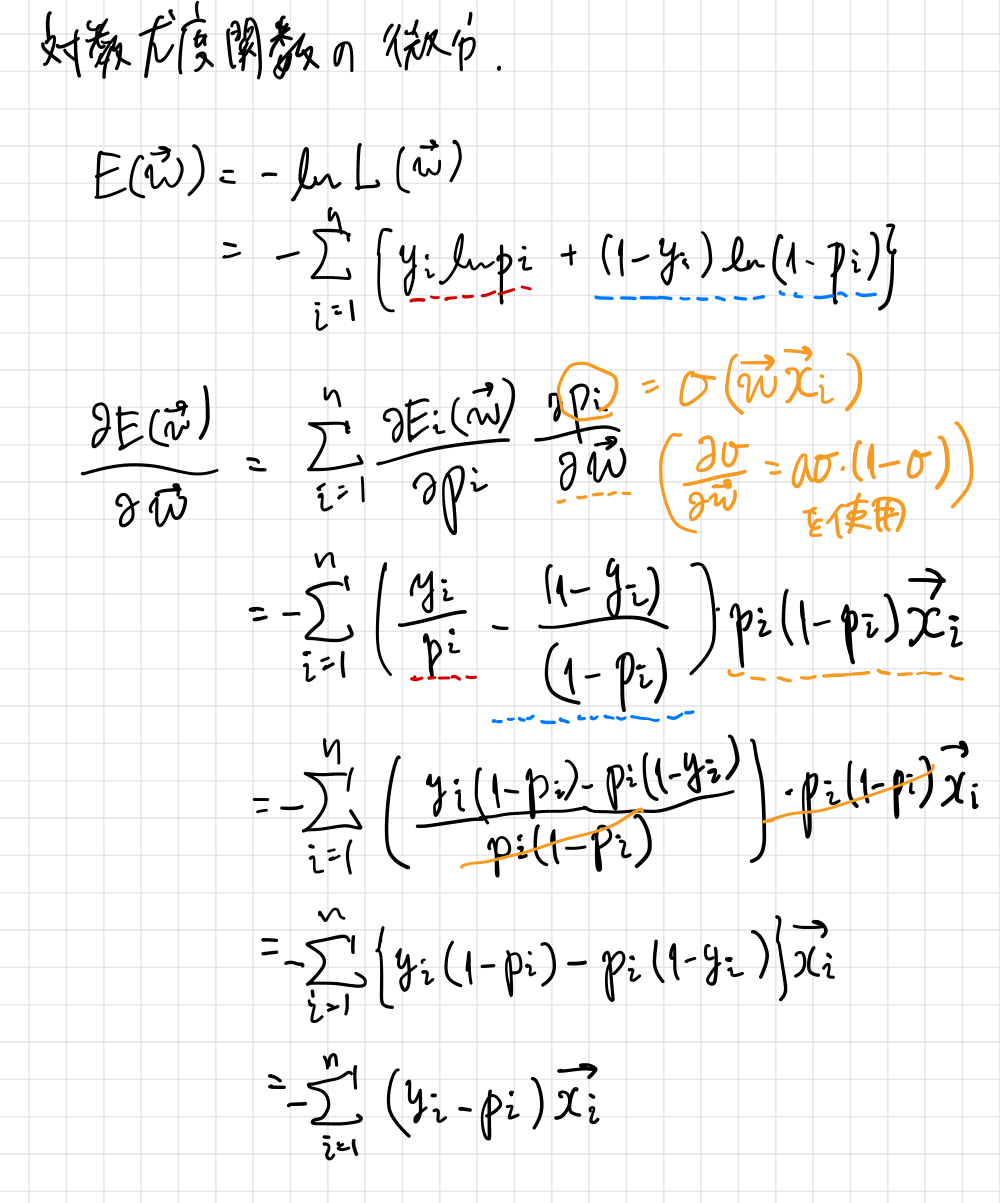
\includegraphics[width=13cm]{capture/対数尤度関数の微分.png}
  \caption{対数尤度関数の微分}
\end{figure}

\newpage

\subsection{勾配降下法}
反復学習によりパラメータを逐次的に更新するアプローチの一つである。勾配降下法は、目的関数の勾配を用いて、目的関数を最小化するようなパラメータを求める方法である。
\begin{align}
  \boldsymbol{w}^{(t+1)} &= \boldsymbol{w}^{(t)} - \eta \frac{\partial E(\boldsymbol{w})}{\partial \boldsymbol{w}} \\
  &= \boldsymbol{w}^{(t)} + \eta \sum^n_{i=1}(\sigma(y_i - p_i)\boldsymbol{x}_i) \label{eq:gd}
\end{align}
で表される。ただし、$\eta$は学習率であり、パラメータの更新量を調整するためのハイパーパラメータである。



\ref{eq:gd}式は、n個のデータを用いてパラメータを更新するため、コンピュータのメモリに対する負荷が大きくなる可能性がある。そのため、データを1つずつ用いてパラメータを更新する方法を確率的勾配降下法(SGD)と呼ぶ。確率的勾配降下法は、データを1つずつ用いてパラメータを更新するため、計算コストが低いという利点がある。ただし、収束が遅くなるという欠点がある。

\newpage

\section{主成分分析}
\subsection{概要}
主成分分析は、多次元データを低次元データに変換する手法である。主成分分析は、データの分散が最大となるような軸を求めることで、データの情報を最大限に保持するような低次元データを求めることができる。

\begin{figure}[htbp]
  \centering
  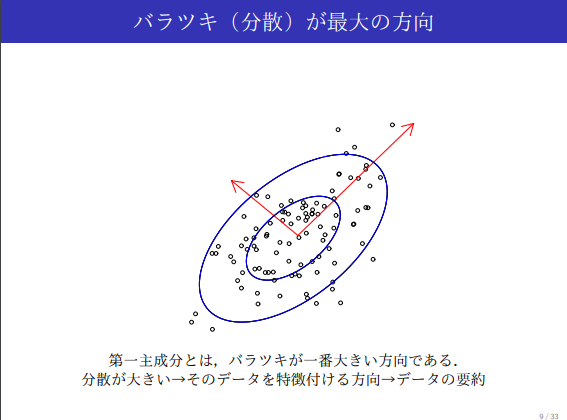
\includegraphics[width=13cm]{main_element.png}
  \caption{主成分分析のイメージ (https://ibis.t.u-tokyo.ac.jp/suzuki/lecture/2015/dataanalysis/L7.pdf より引用)}
\end{figure}

ある方向ベクトルを$\mathbf{v}(||v|| =1)$とおくと、この方向への$\mathbf{x}$の長さは、
\begin{align}
  \mathbf{x}^T\mathbf{v}
\end{align}
で求まる。この分散は、
\begin{align}
  Var(\mathbf{x}^T\mathbf{v}) &= \frac{1}{n-1} \sum_{i=1}^{n}\left[ \mathbf{v}^T (\mathbf{x_i}- \hat{\mu}) \right]^2 \\
  &= \mathbf{v}^T \left( \frac{1}{n-1} \sum_{i=1}^{n} (\mathbf{x_i}- \hat{\mu})(\mathbf{x_i}- \hat{\mu})^T \right) \mathbf{v}\\
  &=: \mathbf{v}^T \mathbf{\Sigma} \mathbf{v} 
\end{align}
で表される。この時、$\mathbf{\Sigma}$は、データの共分散行列である。この分散を最大にするような$\mathbf{v}$を求めることが、主成分分析の目的である。

\newpage

\section{k近傍法}
\subsection{概要}
k近傍法は、分類問題や回帰問題において、新しいデータが与えられた時に、そのデータに最も近いk個のデータを用いて、そのデータがどのクラスに属するかを予測する手法である。
k近傍法には、kd-tree、近似最近傍探索といった手法が存在する。
\par
kが小さいとき、より局所的な情報を用いるため、識別面が入り組んだ形状となる。一方で、kが大きいとき、より大域的な情報を用いるため、識別面が滑らかな形状となるが、kをあまりにも大きくすると、識別精度が下がったり、距離計算のコストが大きくなるという欠点がある。
\par
また、高次元の空間では、データのフィルタリングと精度のバランスをとることが重要である。その際に近似最近傍探索を用いることで、計算コストを削減することができる。その一つがkd-treeである。
\par
kd-treeは、データを分割することで、データの探索を効率化する手法である。kd-treeは、データを分割する際に、データの分散が最大となるような軸や、データの中央値を選択し、データを分割する。この操作を繰り返すことで、データを高速・効率的に探索することができる。
ただし、高次元の計算には適さず、あくまで多次元のデータに対して適している。

\subsection{距離計算}
k近傍法において、データ間の距離を計算する方法には、コサイン距離、ユークリッド距離、マンハッタン距離、Lp距離、マハラノビス距離などがある。
\begin{figure}[htbp]
  \centering
  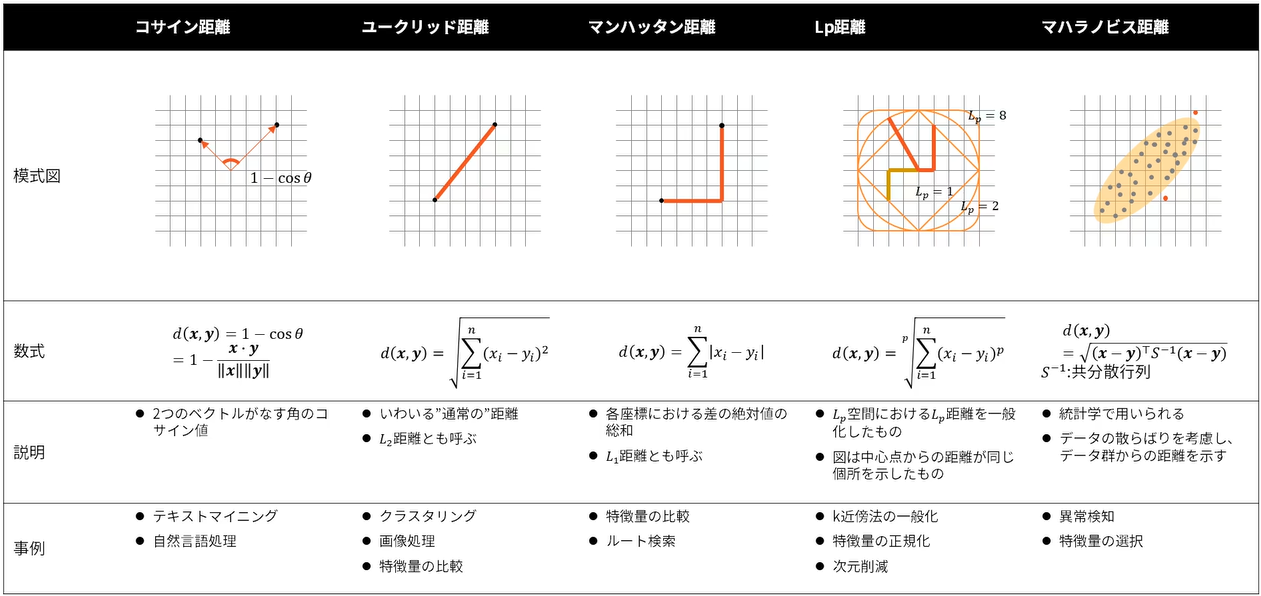
\includegraphics[width=13cm]{capture/距離計算.png}
  \caption{距離計算の手法}
\end{figure}


\newpage

\section{k-means法}
\subsection{概要}
k-means法は、教師なし学習のクラスタリング手法の一つで、データをk個のクラスタに分割する手法である。k-means法は、各クラスタの中心を求め、各データが最も近いクラスタに割り当てることで、データをクラスタに分割する。
初期値が近いと上手くクラスタリングできないことがあるため、複数回の初期値設定を行い、最も良いクラスタリング結果を選択する方法がある。
\subsection{k-means++}
k-means法は初期値に応じて、結果が大きく変わることがある。そのため、初期値を適切に設定することが重要な要素となる。
k-means++は、k-means法における初期値依存問題の克服を目指したアルゴリズムである。
k-means++は初期のクラスタの中心同士が離れていた方がよい、という考え方に基づいて設計されている。
クラスタの割り振り方は、以下の通りである。
\begin{enumerate}
  \item 各データ点$x_i$の中からランダムに1点を選び、クラスタ中心とする
  \item 各点$x_i$に関して、既存のクラスタ中心の中から最も近いクラスタ中心との距離$D(x)$を計算する
  \item 各点$x_i$に関して、重み付き確率分布$P(x_i) = \frac{D(x_i)^2}{\sum_{j}D(x_j)^2}$に従って、新たなクラスタ中心を選ぶ。ただし、$j$は既存のクラスタ中心のインデックスである。
  \item 2.と3.の工程をクラスタ中心が選定できるまで行う
\end{enumerate}
ポイントは、重み付き確率分布$\frac{D(x_i)^2}{\sum_{j}D(x_j)^2}$の確率が最も高くなる場所は、既存のクラスタ中心から最も遠い点になるということである。
以下に、k-means++の初期化のアルゴリズムを示す。

\begin{itembox}[l]{}
  \begin{verbatim}
    probabilities = np.repeat(1/n, n)
    centroids = np.zeros((k, 2))
    distances = np.zeros((n, k))

    for i in range(k):
        centroids[i] = X[np.random.choice(np.arrange(n), p=probabilities, size=(1))]
        distances[:, i] = np.sum((data - centroids[i])**2, axis=1)
        # ある点が次のクラスタ中心になりうる確率 = (ある点の各クラスタからの距離の合計)/(すべての点の各クラスタからの距離の合計)
        probabilites = np.sum(distances, axis=1)/np.sum(distances) 
        
  \end{verbatim}
\end{itembox}

\section{SVM(サポートベクターマシン)}
\subsection{概要}
SVMは、分類問題において、データを2つのクラスに分類する手法である。SVMは、データを分割する直線を決定するため、最適な直線を求めることが目的である。
SVMは、マージン最大化という考え方に基づいており、データを分割する直線と、その直線に最も近いデータとの距離が最大となるような直線を求めることが目的である。
SVMは、線形SVMと非線形SVMに分けられる。線形SVMは、データを分割する直線が直線である場合であり、非線形SVMは、データを分割する直線が曲線である場合である。

\subsection{カーネル法}
非線形SVMにおいて、トレーニングデータを射影関数$\phi$を使って高次元の特徴空間に射影して学習し、学習後に同じ射影関数$\phi$を使って元に戻して解く方法をカーネル法と呼ぶ。
\begin{align}
  f(x) &= b + \sum_{i=1}^{m} \alpha_i x^T x^{(i)} \\
&= b + \sum_{i=1}^{m} \alpha_i \cdot \phi(x) \cdot \phi(x^{(i)})
\end{align}
ただし、$\alpha_i$は、ラグランジュ乗数である。
この方法は、射影する特徴空間の次元数が非常に高くなってしまうことが多く、新しい特徴量 $\phi(x), \phi(x^{(i)})$を生成する計算コストが非常に高くなってしまう。そこで、射影関数の内積結果$\phi(x) \cdot \phi(x^{(i)})$ を既知の変数だけで計算する手法をカーネルトリックと言い、その条件を満たす関数$f(x,x^{(i)}) = \phi(x) \cdot \phi(x^{(i)})$
をカーネル関数と呼ぶ。

代表的なカーネル関数は、以下の通りである。
\begin{itemize}
  \item 多項式カーネル: $K(x^{(i)}, x^{(j)}) = (x^{(i)T} x^{(j)} + c)^d$
  \item ガウシアンカーネル: $K(x^{(i)}, x^{(j)}) = \exp(-\frac{||x^{(i)} - x^{(j)}||^2}{2\sigma^2})$
  \item シグモイドカーネル: $K(x^{(i)}, x^{(j)}) = \tanh(\alpha x^{(i)T} x^{(j)} + c)$
\end{itemize}



\paragraph{参考文献}
\begin{enumerate}
  \item 機械学習・自然言語処理の勉強メモ- 識別モデルと生成モデル (https://kento1109.hatenablog.com/entry/2018/01/10/111249) 2024年4月21日閲覧
  \item k-means++を理解する (@g\-k) (https://qiita.com/g-k/items/e1d558ffcdc833e6382c) 2024年6月11日閲覧
  \item カーネル関数って結局なんなの?→サンプル間の類似度と理解するのがよいと思います! \url{https://datachemeng.com/what_is_kernel/}
  \item 機械学習/カーネル法 (@jun40vn) (https://qiita.com/jun40vn/items/07c3b4d242f3e7e66265) 2024年6月19日閲覧
\end{enumerate}


\newpage

\end{document}